\documentclass{beamer}
\usepackage[orientation=portrait,width=30in,height=40in,scale=1.35,debug]{beamerposter}
\mode<presentation>{\usetheme{ZH}}
\usepackage{chemformula}
\usepackage[utf8]{inputenc}
\usepackage[english]{babel} % required for rendering German special characters
\usepackage{hyperref} %enable hyperlink for urls
\usepackage{ragged2e}
\usepackage[font=footnotesize, justification=justified]{caption}
\usepackage{array,booktabs,tabularx}
\usepackage{bm}
\usepackage{subcaption}

\def\ci{\perp\!\!\!\!\!\perp}

\newcolumntype{Z}{>{\centering\arraybackslash}X} % centered tabularx columns
\title{\huge A Simple Unified Approach to Testing High-Dimensional Conditional Independencies for Ordinal and Categorical Variables}
\author{Ankur Ankan, Johannes Textor}
\institute[RU]{Institute for Computing and Information Sciences \\ Radboud University, Netherlands}
\date{\today}

% edit this depending on how tall your header is. We should make this scaling automatic :-/
\newlength{\columnheight}
\setlength{\columnheight}{104cm}

\begin{document}
\begin{frame}
\begin{columns}
	\begin{column}{.33\textwidth}
		\begin{beamercolorbox}[center]{postercolumn}
			\begin{minipage}{.98\textwidth}  % tweaks the width, makes a new \textwidth
				\parbox[t][\columnheight]{\textwidth}{ % must be some better way to set the the height, width and textwidth simultaneously
					\begin{myblock}{Introduction}
						\begin{figure}
							\begin{subfigure}{0.46\textwidth}
								\centering
								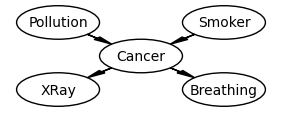
\includegraphics[scale=1.5]{../in_person/imgs/example_dag.png}
							\end{subfigure}%
							\begin{subfigure}{0.08\textwidth}
								$$ \bm{\implies} $$
							\end{subfigure}%
							\begin{subfigure}{0.46\textwidth}
								\begin{equation*}
									\begin{split}
										\text{\emph{XRay}} \ci & \text{\emph{Pollution}} | \text{\emph{Cancer}} \\
										\text{\emph{Breathing}} \ci & \text{\emph{Smoker}} | \text{\emph{Cancer}} \\
										& \vdots \\
									\end{split}
								\end{equation*}
							\end{subfigure}
							\caption*{Example of Causal Markov Condition in a DAG \footnotemark}
						\end{figure}

	\begin{itemize}
		\item In applied research, most of the DAGs are constructed by
			hand based on domain knowledge. Hence, it is important
			to test whether the theorized model is consistent with
			the data. Conditional Independence (CI) tests can be
			used to test these models by verifying whether the
			implied CIs of the model are valid in the data or not.
		\item Constraint-Based structure learning algorithms like PC and FCI exploit
			the CI in the data to construct the model skeleton. They start with
			a fully connected network, and iteratively remove edges if the variables 
			are independent given some of their neighbours.
			% CI implies that no direct causal link exists between the variables.
			% $$ \text{\emph{XRay}} \ci \text{\emph{Smoker}} | \text{\emph{Cancer}} \implies \text{No edge b/w \emph{XRay} and \emph{Smoker}} $$
	\end{itemize}

					\end{myblock}\vfill
					\begin{myblock}{Current Approaches to CI Testing}
						\begin{itemize}
							\item \textbf{Stratification based tests}: Converts CI
								test into a set of non-conditional independence tests
								by splitting the dataset into smaller datasets corresponding to
								every possible value for conditional variables, and finally combines 
								the results. This approach is commonly used for discrete variables, and
								the main drawback is that it looses power quickly as the number of conditional variables
								is increased.

								% $$ D[X, Y, \bm{Z}] = \{ D[X, Y, \bm{Z}=\bm{z_1}], D[X, Y, \bm{Z}=\bm{z_2}], \cdots \} $$
								% \begin{itemize}
								% 	\item Commonly used for discrete variables.
								% 	\item Looses power quickly with increasing number of conditional variables.
								% \end{itemize}
							\item \textbf{Variable Importance based tests}: Uses two
								probability estimators $ \hat{p}(x | y, z) $ and $
								\hat{p}(x | z) $, and compares the goodness of fit.
								If the simpler model does fit worse, it implies independence
								between the variables. A benefit is that any estimator with a 
								goodness of fit measure can be used but these are inherently asymmetrical.
							\item \textbf{Residualization based tests}: Uses two estimators $
								\mathbb{E}[X | Z] $ and $ \mathbb{E}[Y|Z] $, and tests
								for multiplicative association between the residuals \cite{Daudin1980}. Any unbaised
								estimator can be used and is also symmetrical. But residuals
								aren't easy to define for categorical/ordinal variables.

								% \begin{itemize}
								% 	\item Any estimator can be used.
								% 	\item Symmetric.
								% 	\item No such test exists for categorical variables.
								% \end{itemize}
						\end{itemize}
					\end{myblock}\vfill
					\begin{myblock}{Proposed Test}
						\begin{itemize}
							\item \textbf{Estimator:} Asymptotic results require the
								estimators to be M-Estimators (e.g. Generalized Linear
								Model (GLM)). But in empirical analysis, we show that it works with non M-Estimators as well.
							\item \textbf{Residuals:} Li-Shepherd (LS) residuals \cite{li2012}.
								Given an ordinal variable $ Y $ and an estimate $ \hat{p}(y) $ of $
								p(y) $, LS-Residual for sample $ y_i $ is defined as:
								$$ R_{y_i} = \hat{p}(Y < y_i) - \hat{p}(Y > y_i) $$

								For the binary case with $ Y \in \{0, 1\} $:
								$$ R_{y_i} = y_i - \hat{p}(Y = 1) $$

								For the conditional case for sample $ (y|z)_i $,
								$$ R_{y_i | z_i} = \hat{p}(Y < y_i | Z=z_i) - \hat{p}(Y>y_i|Z=z_i) $$
							\item \textbf{Test Statistic:} Hotelling's $ T^2 $ test (a
								multidimensional location test) on residual products.
						\end{itemize}
					\end{myblock}\vfill
		}\end{minipage}\end{beamercolorbox}
	\end{column}
	\begin{column}{.33\textwidth}
		\begin{beamercolorbox}[center]{postercolumn}
			\begin{minipage}{.98\textwidth} % tweaks the width, makes a new \textwidth
				\parbox[t][\columnheight]{\textwidth}{ % must be some better way to set the the height, width and textwidth simultaneously
					\begin{myblock}{Test Statistic}
						\begin{itemize}
							\setlength\itemsep{0.5em}
							\item \textbf{Both Ordinal Variables:}
							$$ Q_1(\bm{x}, \bm{y}) = \frac{1}{n} \frac{(R_{\bm{x}} \cdot R_{\bm{y}})^2}{\bm{var}(R_{\bm{x}} R_{\bm{y}})} $$
							If $ X \ci Y | Z $, asymptotically $ Q_1 \sim \chi^2(1) $.
							\item \textbf{One Ordinal and One Categorical Variable:}
										$$ Q_2(\bm{x}, \bm{y}) = \frac{1}{n} (d \times \hat{\Sigma}_d^{-1} \times d^T) $$
										$$ d = (R_{\mathbb{I}(\mathbf{x}=1)} \cdot R_{\mathbf{y}}, \, \ldots \ , R_{\mathbb{I}(\mathbf{x}=k-1)} \cdot R_{\mathbf{y}}) $$
								If $ X \ci Y | Z $, asymptotically $ Q_2 \sim \chi^2(k-1) $.
							\item \textbf{Both Categorical Variables:}
							\begin{equation*}
								\begin{split}
									& Q_3(\bm{x}, \bm{y}) = \frac{1}{n} (d \times \hat{\Sigma}_d^{-1} \times d^T) \\
								d = (&R_{\mathbb{I}(\mathbf{x}=1)} \cdot R_{\mathbb{I}(\mathbf{y}=1)}, \, \ldots \ ,
										R_{\mathbb{I}(\mathbf{x}=k-1)} R_{\mathbb{I}(\mathbf{y}=1)}, \, \ldots \, , \\
								     &R_{\mathbb{I}(\mathbf{x}=1)} \cdot R_{\mathbb{I}(\mathbf{y}=r-1)}, \, \ldots \ ,
										R_{\mathbb{I}(\mathbf{x}=k-1)} R_{\mathbb{I}(\mathbf{y}=r-1)}) 
								\end{split}
							\end{equation*}
							
							If $ X \ci Y | Z $, asymp. $ Q_3 \sim \chi^2((k-1)(r-1)) $.
						\end{itemize}

					\end{myblock}\vfill
					\begin{myblock}{Empirical Analysis}
						\begin{figure}
							\centering
							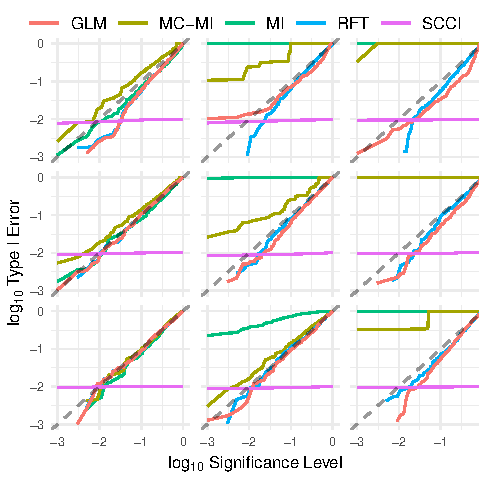
\includegraphics[scale=3]{../in_person/imgs/calibration_add_vars.pdf}
							\caption{Type I error vs significance level for sample sizes (top to
							bottom): $ [20, 40, 80] $ and number of conditional variables (left to
							right): $ [1, 3, 5] $ on conditionally independent simulated binary
							datasets.}
							\label{fig:calibration}
						\end{figure}
						\begin{figure}
							\centering
							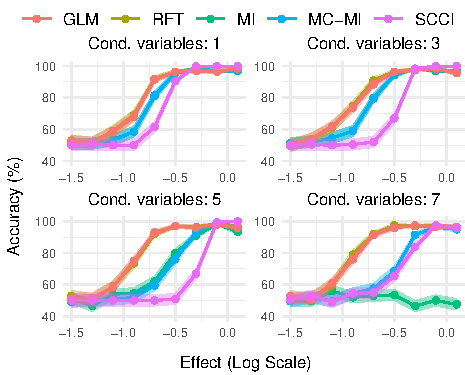
\includegraphics[scale=3]{../in_person/imgs/accuracy.pdf}
							\caption{Accuracy (shading: mean $\pm$ standard error, $N=200$) of classifying
							simulated binary datasets (sample size: $1000$) as conditionally
							dependent or independent.}
							\label{fig:cat_discrimination}
						\end{figure}
						\begin{figure}
							\centering
							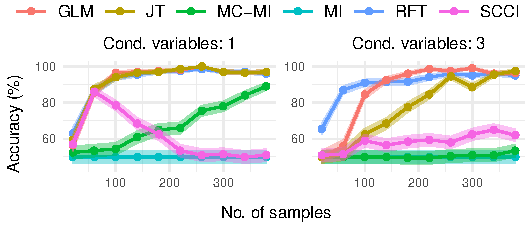
\includegraphics[scale=3]{../in_person/imgs/accuracy_ordinal.pdf}
							\caption{Accuracy (shading: mean $\pm$ standard error, N=200) of
								classifying simulated ordinal data (8 levels per variable) as
								conditionally dependent or independent.}
							\label{fig:accuracy_ord}
						\end{figure}
					\end{myblock}
		}\end{minipage}\end{beamercolorbox}
	\end{column}
	\begin{column}{0.33\textwidth}
		\begin{beamercolorbox}[center]{postercolumn}
			\begin{minipage}{.98\textwidth} % tweaks the width, makes a new \textwidth
				\parbox[t][\columnheight]{\textwidth}{ % must be some better way to set the the height, width and textwidth simultaneously
					\begin{myblock}{Empirical Analysis Cont.}
						\begin{figure}
							\centering
							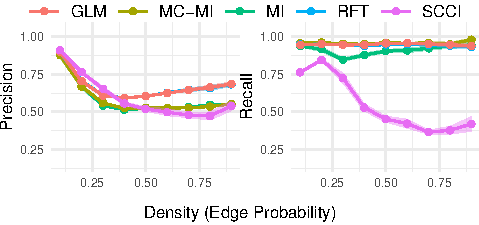
\includegraphics[scale=3]{../in_person/imgs/model_testing.pdf}
							\caption{Precision and recall of testing implied versus non-implied CIs
								 in binary data (N=1000) simulated from random DAGs on $ 20 $ variables.
								 Shading: mean $\pm$ standard error.} 
							\label{fig:model_testing}
						\end{figure}
						\begin{figure}
							\centering
							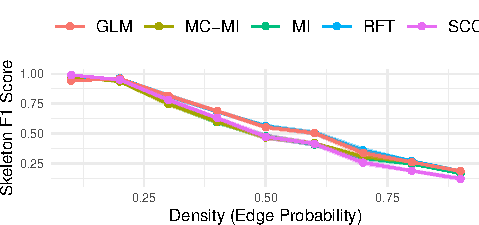
\includegraphics[scale=3]{../in_person/imgs/sl_density.pdf}
							\caption{Structure learning on simulated data: Mean F1 scores (10
								 simulated binary datasets per point) for varying graph densities. Each
								 dataset contains 1000 samples and is simulated from a randomly
								 generated DAG with 20 variables. Shading: mean $\pm$ standard error.}
							\label{fig:sl_density}
						\end{figure}
						\begin{figure}
							\centering
							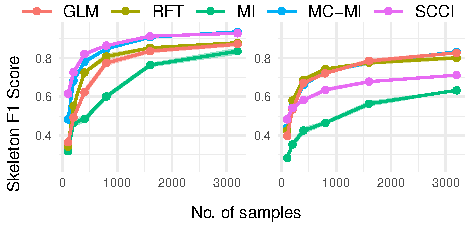
\includegraphics[scale=3]{../in_person/imgs/sl.pdf}
							\caption{Structure learning on datasets ``alarm'' (left) and ``insurance'' (right):
								Mean F1~scores (10 subsampled datasets per sample size) of the learned
								model skeletons.  Presence of an edge is considered the ``positive'' case
								for F1~scores. Shading: mean $\pm$ standard error.}
							\label{fig:sl}
						\end{figure}
						\begin{figure}
							\centering
							\begin{subfigure}[b]{0.6\columnwidth}
								\centering
								\begin{tikzpicture}[scale=5]
									\tikzstyle{every node}=[inner sep=1pt, align=center]
									\scriptsize
									\node (hrpw) at (0:1.2cm) {HrPW};
									\node (race) at (-33:1.2cm) {Race};
									\node (ntvc) at (-61:1.2cm) {NtvC};
									\node (edct) at (-98:1.2cm) {Edct};
									\node (age) at (-131:1.2cm) {Age};
									\node (mrts) at (-164:1.2cm) {MrtS};
									\node (rltn) at (-196:1.2cm) {Rltn};
									\node (sex) at (-225:1.2cm) {Sex};
									\node (occp) at (-262:1.2cm) {Occp};
									\node (incm) at (-300:1.2cm) {Incm};
									\node (wrkc) at (-333:1.2cm) {Wrkc};
						
									\draw [] (hrpw) -- (race) -- (ntvc) -- (edct) -- (age) -- 
										(mrts) -- (rltn) -- (sex) -- (occp) -- (incm) -- (wrkc) -- (hrpw);
						
									\draw [] (hrpw) -- (incm) -- (age) -- (hrpw);
						
									\draw [] (wrkc) -- (edct) -- (occp) -- (wrkc);
						
									\draw [] (edct) -- (rltn) -- (age);
						
									\draw [] (hrpw) -- (edct) -- (incm);
								\end{tikzpicture}
								\caption{}
								\label{fig:sl_adult_model}
							\end{subfigure}%
							\begin{subfigure}[b]{0.4\columnwidth}
								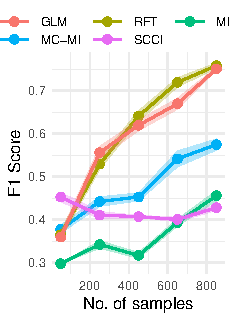
\includegraphics[scale=2.7]{../in_person/imgs/adult_F1.pdf}
								\caption{}
								\label{fig:sl_adult}
							\end{subfigure}
							\caption{Structure learning on adult income data. (a) Skeleton
								estimated by the stable PC algorithm from the data in
								Figure~\ref{fig:pcerror} when using our Random-Forest based
								test (RFT). (b) Mean F1 score ($10$ adult income data subsamples
								per point)
								when comparing $d$-connected variable pairs in the CPDAG to
								correlated variable pairs in the dataset. Presence of
								d-connection is used as the positive case for the
								F1 score. Shading: mean $\pm$ standard
								error.}
						\end{figure}
					\end{myblock}\vfill
					\begin{myblock}{Conclusion}
						\begin{itemize}
							\item A residualization based CI test that works for a
								combination of ordinal and categorical variables.
							\item Properties: 1) Simple to implement; 2) Interpretable
								chi-square test statistic; 3) Symmetric by
								construction; 4) Computationally feasible
							\item Performs reasonably well for low number of conditional
								variable but performs better for high number of
								conditional variables.
							\item For structure learning, a hybrid approach can be used
								with other tests.
							\item Estimators like Random Forests can work with combination
								of discrete and continuous variables, can possibly be
								extended to a single unified test for all data types.
						\end{itemize}
					\end{myblock}\vfill
					\begin{myblock}{References}
						\footnotesize
						\bibliographystyle{abbrv}
						\bibliography{./bib}
					\end{myblock}\vfill
		}\end{minipage}\end{beamercolorbox}
	\end{column}
\end{columns}
\end{frame}
\end{document}
